\begin{tikzpicture}[x=1cm,y=1cm,font=\small]
  % Z = 2.4, Q = 2 (Z = 1.2 Q); C = 0.44
  \def\Zh{1.2}\def\Q{2}\def\C{0.44}
  \draw[->] (-6.6,0) -- (6.9,0) node[right] {$a$};
  % bin edges
  \foreach \s in {-1,1} {
    \foreach \i in {0,1,2} {
      \pgfmathsetmacro{\e}{\s*(\Zh+\i*\Q)}
      \draw (\e,-0.18) -- (\e,0.18);
    }
  }
  \node[below=1mm,font=\footnotesize] at (\Zh,-0.12) {$\tfrac{Z}{2}$};
  \node[below=1mm,font=\footnotesize] at (-\Zh,-0.12) {$-\tfrac{Z}{2}$};
  \node[below=1mm,font=\footnotesize] at (\Zh+\Q,-0.12) {$\tfrac{Z}{2}{+}Q$};
  \node[below=1mm,font=\footnotesize] at (-\Zh-\Q,-0.12) {$-\tfrac{Z}{2}{-}Q$};
  % indices
  \node at (0,0.55) {$p=0$};
  \foreach \i in {1,2} {
    \pgfmathsetmacro{\c}{\Zh+(\i-0.5)*\Q}
    \node at (\c,0.55) {$p=\i$};
    \node at (-\c,0.55) {$p=-\i$};
  }
  \node at (6.1,0.55) {$\cdots$};
  \node at (-6.1,0.55) {$\cdots$};
  % reconstruction points (p - C) Q + Z/2
  \foreach \i in {1,2} {
    \pgfmathsetmacro{\r}{(\i-\C)*\Q+\Zh}
    \fill (\r,0) circle (0.07);
    \fill (-\r,0) circle (0.07);
  }
  \fill (0,0) circle (0.07);
  % braces
  \draw[decorate,decoration={brace,amplitude=4pt,mirror}] (-\Zh,-0.75) -- (\Zh,-0.75)
    node[midway,below=4pt,font=\footnotesize] {zero bin, width $Z$};
  \draw[decorate,decoration={brace,amplitude=4pt,mirror}] (\Zh+\Q,-0.75) -- (\Zh+2*\Q,-0.75)
    node[midway,below=4pt,font=\footnotesize] {width $Q$};
  \pgfmathsetmacro{\ra}{(1-\C)*\Q+\Zh}
  \draw[densely dotted] (\ra,0) -- (\ra,-1.55) node[below,font=\footnotesize] {$\hat a = (1-C)\,Q + \tfrac{Z}{2}$};
\end{tikzpicture}
